% GENERATED by scripts/paper/figures.py -- do not edit by hand.
\begin{figure}[t]
\centering
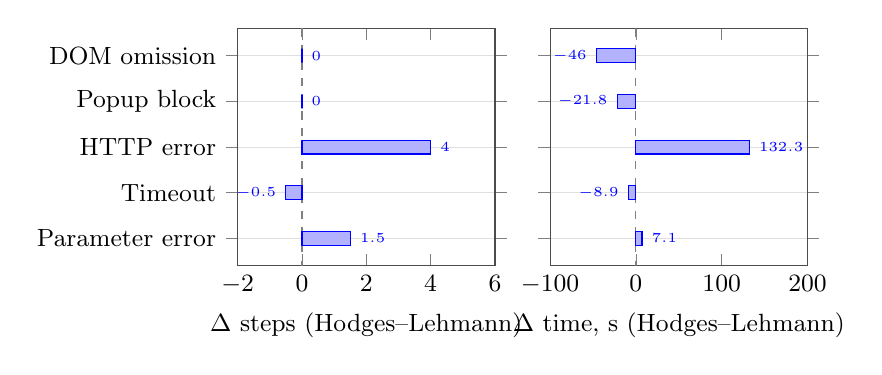
\begin{tikzpicture}
\begin{axis}[name=steps, xbar, bar width=5pt,
  width=0.40\linewidth, xmin=-2, xmax=6,
  ytick={1,2,3,4,5}, y dir=reverse, ymin=0.4, ymax=5.6,
  height=4.6cm,
  tick label style={font=\small}, label style={font=\small},
  nodes near coords, nodes near coords style={font=\tiny},
  ymajorgrids, grid style={gray!25},
  yticklabels={{DOM omission},{Popup block},{HTTP error},{Timeout},{Parameter error}},
  xlabel={$\Delta$ steps (Hodges--Lehmann)},
  fill=gray!60, draw=black!70,
]
\draw[gray,dashed] (axis cs:0,0.4) -- (axis cs:0,5.6);
\addplot coordinates {(0.0,1) (0.0,2) (4.0,3) (-0.5,4) (1.5,5)};
\end{axis}
\begin{axis}[name=time, at={(steps.east)}, anchor=west, xshift=0.7cm,
  xbar, bar width=5pt, width=0.40\linewidth, xmin=-100, xmax=200,
  ytick={1,2,3,4,5}, y dir=reverse, ymin=0.4, ymax=5.6,
  height=4.6cm,
  tick label style={font=\small}, label style={font=\small},
  nodes near coords, nodes near coords style={font=\tiny},
  ymajorgrids, grid style={gray!25},
  yticklabels={},
  xlabel={$\Delta$ time, s (Hodges--Lehmann)},
  fill=gray!60, draw=black!70,
]
\draw[gray,dashed] (axis cs:0,0.4) -- (axis cs:0,5.6);
\addplot coordinates {(-46.0,1) (-21.8,2) (132.3,3) (-8.9,4) (7.1,5)};
\end{axis}
\end{tikzpicture}
\caption{Within-pair process cost on the behavioural matrix. HTTP errors and parameter errors cost the agent steps and time, while DOM omission and popup blocking make it \emph{faster} --- which we read as fault-induced early termination. All five are significant at $p<0.01$ except where noted in Table~\ref{tab:behavior}.}
\label{fig:behavior}
\end{figure}
